
\chapter{Essential reading for users of MLS version~\thisv data}
\label{chap:Essential}

\section{Scope and background for this document}

This document describes the quality of the geophysical data products produced by version~6.0 of the data processing algorithms for the Earth Observing System (EOS) Microwave Limb Sounder (MLS) instrument on NASA's Aura spacecraft. The intended audience is those wishing to make use of Aura MLS data for scientific study. This chapter, as its name implies, is considered essential reading for all users of MLS data.

Chapter~\ref{chap:Background} provides additional optional background information, outlining the algorithms used to generate the ``Level~2'' data (geophysical products reported along the instrument track) from the input ``Level~1'' data (calibrated microwave radiance observations). The bulk of the document, in Chapter~\ref{chap:Results}, provides information on each of the MLS standard ``Level~2'' products. This includes quantification of resolution, precision, and accuracy, along with a description of data screening and usage rules and other caveats, notes on any anomalies, and some limited comparisons to other datasets. Key aspects of each product are summarized in Table~\ref{tab:ProductSummary}. Finally, Chapter~\ref{chap:Level3} (added in version 4.x-4.0 of this document) describes ``Level~3'' data products, derived from the Level~2 data, that provide easier access to collections of MLS observations (e.g., daily zonal means, monthly polar vortex averages) to facilitate additional studies using MLS observations. Users of these Level~3 data should still read the Chapter~\ref{chap:Essential} material and the product-specific information in Chapter~\ref{chap:Results}.

The \thisv MLS data are the sixth ``public release'' of MLS data, having been preceded by versions~1.5, 2.2, 3.3/3.4, 4.2, and 5.0\@. The v2.2 data are described in a series of validation papers published in a special issue of the \emph{Journal of Geophysical Research} in 2007/2008. This document updates some findings from these papers for \thisv, compares a limited subset of available \thisv results to some of the previous data versions, and gives more general information on the use of MLS data. As always, those wishing to use MLS data are advised to consult the MLS science team concerning their intended use.

%
\newenvironment{tablenotes}{%
  \begin{list}{}{%
      \renewcommand{\makelabel}[1]{##1}%
      \setlength{\itemsep}{0.5ex}%
      \setlength{\topsep}{0.5ex}%
      \setlength{\parskip}{0pt}%
      \setlength{\partopsep}{0pt}%
      \setlength{\parsep}{0pt}%
      \setlength{\itemindent}{0em}%
      \setlength{\leftmargin}{1.5em}%
      \setlength{\labelwidth}{1.5em}%
      \setlength{\labelsep}{0pt}%
    }}%
  {\end{list}}
\newcommand{\tabnudge}[1]{\smash{\raisebox{1.4ex}{#1}}}
%
\begin{table}
\renewcommand{\thefootnote}{\sffamily[\arabic{footnote}]}
\renewcommand{\arraystretch}{1.3}
%
\caption{Summary of key information for each MLS standard product.
  Essential additional information is given in each product section of
  chapter~\ref{chap:Results}.}
\label{tab:ProductSummary}
\vspace{-2mm}
%
\begin{center}
\small\sffamily
\begin{tabular}{lllllll}
\toprule
\rule[-2.5ex]{0pt}{6ex}\textbf{Product name} & 
\parbox{2.5cm}{\raggedright\bfseries Useful vertical range~/~hPa} &
\parbox{2.2cm}{\raggedright\bfseries \texttt{Quality} threshold\,\footnotemark[1]} &
\parbox{2.2cm}{\raggedright\bfseries \texttt{Convergence} threshold\,\footnotemark[2]} &
\textbf{Notes} &
\textbf{Contact name} \\
\midrule
%
\flipfloprow
\hyperref[sec:StandardBrO]{\texttt{BrO}} & 10\,--\,3.2 & 1.3 & 1.05 & A,D,N & Luis Mill\'an Valle \\
%
\flipfloprow 
\hyperref[sec:StandardCH3Cl]{\texttt{CH3Cl}} & 147\,--\,4.6 &  1.3 & 1.05 & N & Michelle Santee \\
%
\flipfloprow 
\hyperref[sec:StandardCH3CN]{\texttt{CH3CN}} & 46\,--\,1.0 &  1.4 & 1.05 & E,N & Michelle Santee \\
%
\flipfloprow 
\hyperref[sec:StandardCH3OH]{\texttt{CH3OH}} & \multicolumn{4}{c}{Not to be used pending further validation} & Michelle Santee \\
%
\flipfloprow 
\hyperref[sec:StandardClO]{\texttt{ClO}} & 147\,--\,1.0 & 1.3 & 1.05 & B & Michelle Santee \\
%
\flipfloprow 
& 100\,--\,0.0046 & & & & Hugh Pumphrey \\
\samecolorrow
\tabnudge{\hyperref[sec:StandardCO]{\texttt{CO}}}  & 215\,--\,146 & \tabnudge{1.5} & \tabnudge{1.03} & \tabnudge{C} & Michael Schwartz \\
%
\flipfloprow 
 & 83\,--\,0.001 & 0.2 & & -- &  \\
%
\samecolorrow
\tabnudge{\hyperref[sec:StandardGPH]{\texttt{GPH}}} & 261\,--\,100 & 0.9 & \tabnudge{1.03} & C,O & \tabnudge{Michael Schwartz} \\
%
\flipfloprow & 83\,--\,0.002 & & & -- & Alyn Lambert \\
\samecolorrow
\tabnudge{\hyperref[sec:StandardH2O]{\texttt{H2O}}} & 316\,--\,100 & \tabnudge{1.45} & \tabnudge{2.0} & C &
William Read \\
%
\flipfloprow 
\hyperref[sec:StandardHCl]{\texttt{HCl}} & 100\,--\,0.32 & 1.2 & 1.05 & -- & Lucien Froidevaux \\
%
\flipfloprow 
\hyperref[sec:StandardHCN]{\texttt{HCN}} & 21\,--\,0.1 & 0.2 & 2.0 & A,E,N & Hugh Pumphrey \\
%
\flipfloprow 
\hyperref[sec:StandardHNO3]{\texttt{HNO3}} & 215\,--\,1.5 & See text & See text & C,O & Gloria Manney \\
%
\flipfloprow 
\hyperref[sec:StandardHO2]{\texttt{HO2}} & 22\,--\,0.046 & N/A & 1.1 & A,D,N & Shuhui Wang \\
%
\flipfloprow 
\hyperref[sec:StandardHOCl]{\texttt{HOCl}} & 10\,--\,2.2 & 1.2 & 1.05 & N &  Lucien Froidevaux \\
%
\flipfloprow 
\hyperref[sec:StandardIWC]{\texttt{IWC}} & 215\,--\,83 & N/A & N/A & B & Alyn Lambert \\
%
\flipfloprow 
\hyperref[sec:StandardIWP]{\texttt{IWP}} & N/A & N/A & N/A & B & Alyn Lambert \\
%
\flipfloprow 
\hyperref[sec:StandardN2O]{\texttt{N2O}} & 68\,--\,0.46 & 1.3 & 2.0 & -- & Alyn Lambert \\
%
\flipfloprow 
 & 100\,--\,0.02 & & & & Lucien Froidevaux \\
%
\samecolorrow
\tabnudge{\hyperref[sec:StandardO3]{\texttt{O3}\,\footnotemark[3]}} & 
 261\,--\,121 & \tabnudge{1.0} & \tabnudge{1.03} & \tabnudge{C} &
  Michael Schwartz \\
%
\flipfloprow 
\hyperref[sec:StandardOH]{\texttt{OH}} & 32\,--\,0.0032 & N/A & 1.1 & D & Shuhui Wang \\
%
\flipfloprow 
\hyperref[sec:StandardRHI]{\texttt{RHI}\,\footnotemark[4]} & 316\,--\,0.002 & See text & See text & C,O & William Read \\
%
\flipfloprow 
\hyperref[sec:StandardSO2]{\texttt{SO2}} & 215\,--\,10 & 0.95 & 1.03 & E & William Read \\
%
\flipfloprow 
 & 83\,--\,0.001 & 0.2 & & -- &  \\
%
\samecolorrow
\tabnudge{\hyperref[sec:StandardTemperature]{\texttt{Temperature}\,\footnotemark[5]}} & 261\,--\,100 & 0.9 & \tabnudge{1.03} & C,O & \tabnudge{Michael Schwartz} \\
%
\bottomrule
\end{tabular}
\end{center}
%
\vspace{-2mm}\parbox[t]{0.5\textwidth-0.5\columnsep}{\footnotesize\sffamily
  \textbf{Notes:}\par
  \begin{tablenotes}
  \item[A] Users should consider using alternative versions of this
    product, produced using different algorithms, as described in the text.
  \item[B] This product has significant biases in certain regions
    that may need to be accounted or corrected for in scientific studies.
    See text for details.
  \item[C] Interference from clouds can affect this product at certain
    altitudes. See text for details.
  \item[D] Biases in his product can be ameliorated (in selected
    conditions) by taking day/night differences.  See text.
  \item[E] At some altitudes, this product contains biases of a magnitude
    that render the product useful only for the study of ``enhancement
    events'' (e.g., volcanic plumes, extreme fire pollution).  See text
    for details.
  \end{tablenotes}}%
\hfill\parbox[t]{0.5\textwidth-0.5\columnsep}{\footnotesize\sffamily
  \begin{tablenotes}
  \item[N] This is a ``noisy'' product requiring significant averaging
    (e.g., monthly zonal mean).  See text for details.
  \item[O] This product contains significant outliers (e.g., spikes or
    oscillations) in some regions (typically related to clouds in the
    tropical upper troposphere).  These should be screened out as detailed
    in the text.
  \end{tablenotes}
  \vspace{-1ex}\rule{\linewidth}{0.5pt}\par
  \vspace{-0.5ex}\begin{tablenotes}
  \item[\mbox{[1]}] Only use profiles with \texttt{Quality} \emph{greater}
    than this value.
  \item[\mbox{[2]}] Only use profiles with \texttt{Convergence} \emph{less} than this value.
  \item[\mbox{[3]}] File also contains a swath giving the column
    abundance above the (MLS-defined) tropopause.
  \item[\mbox{[4]}] Relative humidity with respect to ice computed from the
    MLS H\cs2O and Temperature data.
  \item[\mbox{[5]}] File also contains a swath giving tropopause
    pressure (WMO definition) inferred from MLS temperatures.
  \end{tablenotes}}

\end{table}

%%% Local Variables: 
%%% mode: latex
%%% TeX-master: "v4-x-report"
%%% End: 


More information on the MLS instrument can be found in the document \emph{An Overview of the EOS MLS Experiment} \citep{EOSMLSOverview}. A more general discussion of the microwave limb sounding technique and an earlier MLS instrument is given in \citet{WatersEtal:1999}. The theoretical basis for the Level~2 software is described in \citet{EOSMLSL2ATBD}. A crucial component of the Level~2 algorithms is the ``Forward Model'', which is described in detail in \citet{EOSMLSFWMATBD} and \citet{EOSMLSPolarizedFWMATBD}. The document \emph{EOS MLS Retrieved Geophysical Parameter Precision Estimates} \citep{EOSMLSPrecision} provides pre-launch estimates EOS MLS data precision. The impact of clouds on MLS measurements and the use of MLS data to infer cloud properties is described in \cite{EOSMLSCloudATBD}. All the above documents and papers are available from the MLS web site (\url{https://mls.jpl.nasa.gov/}).

A subset of the information in those documents is also reported in a series of articles in the 2006 Aura special issue of the \emph{IEEE Transactions on Geoscience and Remote Sensing}. Specifically, an overview of MLS is given in \cite{WatersEtal:2006}, the algorithms that produce the data described here are reviewed in \citet{LiveseyEtal:2006}, \citet{ReadEtal:2006}, \citet{SchwartzEtal:2006}, and \citet{WuEtal:2006}\@. Other papers describe the calibration and performance of the various aspects of the MLS instrument \citep{JarnotEtal:2006, Pickett:2006, CofieldEtal:2006} and the MLS ground data system \citep{CuddyEtal:2006}. The detailed validation of the MLS v2.2 dataset is described in a collection of papers in the ``Aura Validation'' special issue of JGR-Atmospheres (papers published in 2007 and 2008). These are cited in Chapter~\ref{chap:Results} on a product-by-product basis, along with some more recent references, in some cases.

\section{Overview of \thisv and this document}

The remainder of this chapter reviews issues that are considered \emph{essential reading} for users of the \thisv dataset. Chapter~\ref{chap:Background} details relevant aspects of the MLS instrument design and operations and the theoretical basis for the \thisv Level~2 algorithms that are considered \emph{background reading}.

Chapter~\ref{chap:Results} describes the data quality for ``Standard'' products from the MLS instrument for \thisv. These are observations of vertical profiles of the abundance of BrO, CH\cs3Cl, CH\cs3CN, CH\cs3OH, ClO, CO, H\cs2O, HCl, HCN, HNO\cs3, HO\cs2, HOCl, N\cs2O, O\cs3, and OH and SO\cs2, along with temperature, geopotential height, relative humidity (deduced from the H\cs2O and temperature data), cloud ice water content and cloud ice water path, all described as functions of pressure. These profiles are mostly output on a grid that has a vertical spacing of six surfaces per decade change in pressure (\mytexttilde2.5\,km), thinning out to three surfaces per decade above 0.1\,hPa. Exceptions to this are water vapor, temperature, ozone and relative humidity, which are on a finer 12-per-decade grid from 1000\,hPa to 1\,hPa. Cloud ice water content is also reported on this fine grid, though these profiles do not extend to the stratosphere and mesosphere. The OH product maintains a six-per-decade grid spacing into the upper mesosphere. Horizontally the profiles are spaced by 1.5\degsym\ great-circle angle along the orbit, which corresponds to about 160\,km along track. The true vertical and along-track horizontal resolution of the products is typically somewhat coarser than the reporting grid described here. For some of the products, the signal to noise ratio is too low to yield scientifically useful data from a single MLS profile observation. In these cases, some form of averaging (e.g.,\ weekly maps, monthly zonal means etc.) will be required to obtain more useful results.

In addition to these standard products, the algorithms also produce data for many ``diagnostic'' products. The bulk of these are similar to the standard products, in that they represent vertical profiles of retrieved species abundances. However, the information on these diagnostic products has typically been obtained from a different spectral region than that used for the standard products. These diagnostic products are not discussed in this document. Further information on these is available from the MLS science team.

At the time of writing, the current version of the data processing software is version~6.01, producing files labeled \texttt{v06-01}. Any minor updates for bug fixes, or to reflect changes in input data such as the analysis fields used as \emph{a priori} information for temperature will be referred to as v6.02, v6.03, etc. This version of the document is intended to be applicable to any v6.0\emph{x} data files. More substantial changes at a later date (e.g., due to a change in the MLS instrument performance) may necessitate a larger change in the data processing software and/or its configuration. These will be numbered v6.1\emph{x} etc., and will be accompanied by an updated version of this document (though not necessarily immediately, depending on the circumstances dictating the update).

\section{MLS data validation status}

As discussed above, a complete set of MLS validation papers describes the validation state of the earlier v2.2 data. The majority of the v2.2 MLS data products have, accordingly, completed ``Stage~3 Validation'' defined\footnote{See \url{https://science.nasa.gov/earth-science/earth-science-data/data-maturity-levels/}} as:
%
\begin{quote}
  \itshape Product accuracy has been assessed.  Uncertainties in the product and its associated structure are well quantified from comparison with reference in situ or other suitable reference data. Uncertainties are characterized in a statistically robust way over multiple locations and time periods representing global conditions.  Spatial and temporal consistency of the product and with similar products has been evaluated over globally representative locations and periods.  Results are published in the peer-reviewed literature.
\end{quote}
%
Work, including that described in this document, has re-validated the \thisv data, with the level of scrutiny for some (notably ozone and water vapor) establishing them as ``Stage~4'' validated, defined as:
%
\begin{quote}
  \itshape Validation results for stage~3 are systematically updated when new product versions are released and as the time-series expands.
\end{quote}

\section{Differences between MLS \thisv data and earlier \prevv data}
\label{sec:V5vsV4Overview}

The most significant changes between MLS \thisv data and the previous \prevv dataset at associated with the N\cs2O and Temperature products.  There were also some changes to the way cloud impacts on MLS observations are flagged, and some new cloud metrics were included. In addition to these specific changes, changes in other products have resulted as an indirect response to the temperature changes detailed below. Note that the threshold values of ``\texttt{Quality}'' and ``\texttt{Convergence}'' (see below) to be used in data screening have been updated for some products.

\subsection{sec:V6N2Owork}

As discussed in \citep{LiveseyEtal:2021:Drifts}, the \prevv algorithms included a correction for a long-term drift (of around 1.3\% per decade) in the calibration of the MLS 190-GHz receiver subsystem that started around 2010. This drift led to statistically significant drifts in comparisons between the observations of species measured by this receiver and measurements by other instruments, notably for H\cs2O and N\cs2O. Although the correction applied in \prevv ameliorated the drift in H\cs2O (at least in comparison to ACE-FTS observations), significant issues remained with the N\cs2O product.  The \thisv algorithms include a further correction aimed at ameliorating those issues (see section~\ref{sec:N2OV6Corretion} for more details).  Note that only species measured by the 190-GHz receiver are affected by the drift (specifically H\cs2O, N\cs2O, HCN, and upper stratospheric HNO\cs3).  No other MLS products are impacted.

\subsection{sec:V6TemperatureWork}

The MLS can measure atmospheric temperature profiles by two largely independent means. Firstly, cases where optically thick limb paths are observed convey information on the temperature in the region where the atmosphere becomes opaque.  Secondly, measurements of spectral line shape convey information about atmospheric pressure along the limb ray paths.  By combining this pressure information with knowledge of limb ray path altitude differences (deduced from instrument and spacecraft pointing knowledge), information on temperature profiles can be deduced by assuming atmospheric hydrostatic balance.  Historically, these two approaches have given slightly conflicting information, disagreeing by 1--2\,K \mycomment{Bill, is this correct, or is 1--2\,K only the problems left after we sidestepped the conflict, which might have been bigger?} (which amounts to only a <1\% difference in terms of instrument calibration, within expectations and original instrument requirements). As part the \thisv development, the MLS team modified the spectral shape assumed for channels used to measure the 118\,GHz oxygen line (the main source of MLS temperature information) in order to obtain improved fits to observed radiances.  These adjustments were within the uncertainty reported on pre-launch calibration data, and resulted in better agreement between the two approaches to measuring atmospheric temperature.  This in turn enabled a more-comprehensive use of the MLS radiance signals, improving the precision and vertical resolution of the MLS temperature product from the mid-stratosphere through the mesosphere. \mycomment{correct?}

\subsection{sec:V6CloudWork}

While MLS observations are insensitive to aerosols and thin clouds, the particles and number densities associated with deep convective clouds can lead to scattering of the millimeter-scale signals observed by MLS.  The ima


\section{Aura MLS file formats, contents, and quality information}
\label{sec:FilesAndFormats}
\label{sec:NegativePrecision}

All the MLS Level~2 data files described here are available from the NASA Goddard Space Flight Center Earth Science Data and Information Services Center (GES-DISC, see \url{https://disc.gsfc.nasa.gov/}). The standard and diagnostic products are stored in the EOS MLS \emph{Level 2 Geophysical Product} (L2GP) files. These are standard HDF-EOS (version~5) files containing swaths in the Aura-wide standard format. For more information on this format see \citet{AuraFileConventions}. A sample reading function for the Interactive Data Language (IDL, version 6.1 or later required), known as \texttt{readl2gp.pro} may have been supplied with the data and is available from \url{https://mls.jpl.nasa.gov/data/readers.php} \mycomment{That link doesn't work} A reader for MATLAB (\texttt{readL2GP.m}) is also available at the same site. Standard HDF and NetCDF readers (e.g., in Python, Julia, etc.) are able to read the files as regular HDF-5/NetCDF-4 files (the HDF-EOS ``swaths'' discussed below can be found in the \texttt{HDFEOS/SWATHS} group).

The standard products are stored in files named according to the convention
\begin{quote}
  \verb+MLS-Aura_L2GP-<product>_v06-01-c01_<yyyy>d<ddd>.he5+
\end{quote}
where \verb+<product>+ is \texttt{BrO}, \texttt{O3},
\texttt{Temperature}, etc.  The files are produced on a one-day
granularity (midnight to midnight, universal time), and named
according to the observation date where \verb+<yyyy>+ is the four
digit calendar year and \verb+<ddd>+ is the day number in that year
(\texttt{001} = 1 January).

These files contain the corresponding standard product in an HDF-EOS swath given the same name as the product, e.g., ``\texttt{H2O}''. With the exception of IWC, each file also contains the \emph{a priori} values for that product inside a second swath whose name ends with the substring ``\texttt{-APriori}''. HNO\cs3, IWC, O3, RHI, and Temperature files are special in that they carry extra standard or non-standard products, as detailed in Table~\ref{tab:SwathExtras}.

\begin{table}
  \caption{Additional swaths in specific standard product
    files.\label{tab:SwathExtras}}\small
  \begin{center}
    \begin{tabular}{>{\ttfamily}l>{\ttfamily}ll}
  \toprule
  \textbf{\rmfamily Product} & \textbf{\rmfamily Additional swaths} &
  \textbf{\rmfamily Notes} \\
  \midrule
  HNO3 & HNO3-190, HNO3-240 & Nitric acid from the 190 and
  240\,GHz radiometers\\
  IWC & IWP & partial Ice Water Path.  (This file has no \emph{a priori} swath) \\
  O3 & O3 column & Ozone column above the tropopause (see below) \\
  RHI & UTRHI, UTRHI-APriori & ``Single layer'' relative humidity (see Section~\ref{sec:StandardRHI})\\
  Temperature & WMOTPPressure & Tropopause (WMO definition, based on MLS
  temperature) \\
  \bottomrule
\end{tabular}
  \end{center}
\end{table}

The files contain an HDF-EOS swath given the same name as the product. In addition, the standard O\cs3 product files also contain swaths describing column abundances, and the standard Temperature file contains additional swaths describing tropopause pressure. As some L2GP files contain multiple swaths, it is important to ensure that the correct swath in the \texttt{L2GP} files is requested from the file. In the case where the ``default'' swath is requested (i.e., no swath name is supplied) most HDF software will access the one whose name falls earliest in ASCII order. This generally results in the desired result for all products. For example, for temperature, the standard ``\texttt{Temperature}'' product will be read in preference to the ``\texttt{WMOTPPressure}'' swath that gives tropopause pressures.

Each swath contains data fields \texttt{L2gpValue} and \texttt{L2gpPrecision}, which describe the value and precision (reported at 1$\sigma$) of the data, respectively. Data points for which \texttt{L2gpPrecision} is set negative or zero \emph{should not be used}, as this flags that the resulting precision is worse than 50\% of the \emph{a priori} precision, indicating that instrument and/or the algorithms have failed to provide enough useful information for that point. In addition to these fields, fields such as \texttt{latitude} etc.\ describe geolocation information. The field \texttt{time} describes time, in the EOS standard manner, as the number of seconds (including leap seconds) elapsed since midnight universal time on 1~January 1993.

The \texttt{L2GP-DGG} (``Diagnostic products on a Geophysical Grid'') file contains a large number of additional swath quantities. The vast majority of these are MLS diagnostic products that will be of little interest to most data users. A few that may be of interest to some users are detailed below.

\section{Additional information given in the \texttt{Quality},
  \texttt{Convergence} and \texttt{Status} fields}
\label{sec:StatusQuality}

\usetikzlibrary{calc}
\begin{figure}[tb]
\definecolor{bitcolor}{gray}{0.80}
\newlength{\bitsize}
\setlength{\bitsize}{1.0cm}
\newlength{\meaningheight}
\setlength{\meaningheight}{-1.5cm}
\newlength{\xpos}
\setlength{\xpos}{10.6cm}
\newlength{\ypos}
\setlength{\ypos}{-1.5cm}
\begin{tikzpicture}
\small\sffamily
%
% First the bits
\begin{scope}[minimum size=\bitsize,very thick]
\node (b11) at (0\bitsize,0pt) [rectangle, draw, fill=bitcolor, label=above:10] {\small\ttfamily 1024};
\node (b9) at (1\bitsize,0pt) [rectangle, draw, fill=bitcolor, label=above:9] {\small\ttfamily 512};
\node (b8) at (2\bitsize,0pt) [rectangle, draw, fill=bitcolor, label=above:8] {\small\ttfamily 256};
\node (b7) at (3\bitsize,0pt) [rectangle, draw, fill=bitcolor, label=above:7] {\small\ttfamily 128};
\node (b6) at (4\bitsize,0pt) [rectangle, draw, fill=bitcolor, label=above:6] {\small\ttfamily 64};
\node (b5) at (5\bitsize,0pt) [rectangle, draw, fill=bitcolor, label=above:5] {\small\ttfamily 32};
\node (b4) at (6\bitsize,0pt) [rectangle, draw, fill=bitcolor, label=above:4] {\small\ttfamily 16};
\node (b3) at (7\bitsize,0pt) [rectangle, draw, fill=bitcolor, label=above:3] {\small\ttfamily 8};
\node (b2) at (8\bitsize,0pt) [rectangle, draw, fill=bitcolor, label=above:2] {\small\ttfamily 4};
\node (b1) at (9\bitsize,0pt) [rectangle, draw, fill=bitcolor, label=above:1] {\small\ttfamily 2};
\node (b0) at (10\bitsize,0pt) [rectangle, draw, fill=bitcolor, label=above:0] {\small\ttfamily 1};
% A key
\node at (11\bitsize,0pt) [rectangle, minimum size=\bitsize, label=above:Bit, align=left] {\small\ttfamily\null\hspace{1em} Value};
\end{scope}
%
% Now the meanings
\newcommand{\meaningbox}[2]{\parbox{5cm}{\raggedright\textbf{#1} #2}}
\begin{scope}[inner sep=0pt, outer sep=4pt, anchor=west]
\node (m0) at (\xpos,\ypos+0\meaningheight) {\meaningbox{Flag -- Bad Profile:}%
  {Do not use this profile (see ``information'' bits for an explanation).}};
\node (m1) at (\xpos,\ypos+1\meaningheight) {\meaningbox{Flag -- Warning:}%
  {This profile is questionable (see ``information'' bits for an explanation).}};
\node (m2) at (\xpos,\ypos+2\meaningheight) {\meaningbox{Flag -- Comment}%
  {See ``information'' bits for additional comments concerning this profile.}};
%
% Nudge a bit
%
\addtolength{\ypos}{-2mm}
\node (m4) at (\xpos,\ypos+3\meaningheight) {\meaningbox{Information:}%
  {(Warning) This profile may have been affected by high altitude clouds.}};
\node (m5) at (\xpos,\ypos+4\meaningheight) {\meaningbox{Information:}%
  {(Warning) This profile may have been affected by low altitude clouds.}};
\node (m6) at (\xpos,\ypos+5\meaningheight) {\meaningbox{Information:}%
  {(Comment) GEOS-5 \emph{a priori} temperature data were unavailable for this profile.}};
\node (m7) at (\xpos,\ypos+6\meaningheight) {\meaningbox{Information:}%
  {(Bad profile) The retrieval for this phase encountered a numerical error.}};
\node (m8) at (\xpos,\ypos+7\meaningheight) {\meaningbox{Information:}%
  {(Bad profile) Too few radiances were available for good retrieval of this profile.}};
\node (m9) at (\xpos,\ypos+8\meaningheight) {\meaningbox{Information:}%
  {(Bad profile) The task retrieving this profile crashed (typically a computer failure).}};
\end{scope}
%
% Now a separator
\draw[ultra thick] ($ (m2.west)!0.5!(m4.west) $) -- ($ (m2.east)!0.5!(m4.east) $);
% \draw[ultra thick] (0,0) -- (10,0);
%
% Now the connections
\begin{scope}[>=stealth,thick]
\draw[->] (b0) |- (m0);
\draw[->,dashed] (b1) |- (m1);
\draw[->] (b2) |- (m2);
\draw[->,dashed] (b4) |- (m4);
\draw[->] (b5) |- (m5);
\draw[->,dashed] (b6) |- (m6);
\draw[->] (b7) |- (m7);
\draw[->,dashed] (b8) |- (m8);
\draw[->] (b9) |- (m9);
\end{scope}
\end{tikzpicture}
\caption{The meaning of the various bits in the \texttt{Status} field.
  The bits not labeled are not used in \thisv.  Later versions may
  implement specific meanings for these bits.  Note that bit 6 (GEOS-5
  data) was not used in v1.5, and that the information in bits 7 and 8
  were combined into bit 8 in versions~1.5 and~2.2.}
\label{fig:StatusBits}
\end{figure}


%%% Local Variables: 
%%% mode: latex
%%% TeX-master: "v4-x-report"
%%% End: 


In addition to the data and their estimated precisions, three quality metrics are output for every profile of each product. The first, called \texttt{Quality}, gives a measure of the quality of the product based on the fit achieved by the Level~2 algorithms to the relevant radiances. Larger values of \texttt{Quality} generally indicate better radiance fits and therefore more trustworthy data. Values of \texttt{Quality} closer to zero indicate poorer radiance fits and therefore less trustworthy data. The value of \texttt{Quality} to be used as a ``threshold'' for rejecting data in scientific studies varies from product to product, and is given later in this document.

The second quality metric is called \texttt{Status}. This is a 32 bit integer that acts as a bit field containing several ``flags''. Figure~\ref{fig:StatusBits} describes the interpretation of these flags in more detail. The first three bits (bits 0, 1, and 2) are ``flagging'' bits. If the first bit (``bad profile'') is set it indicates that the profile \emph{should not be used in any scientific study}. Accordingly, any profile for which \texttt{Status} is an odd number should not be used. The second bit (``warning'') indicates that data are considered questionable for some reason, while the third (``comment'') indicates the data are noteworthy in some manner that does not rise to the level of a ``warning''. Higher bits give more information on the reasons behind the setting of the first three bits. So, for example, a value of \texttt{Status} of \texttt{18} (2+16) indicates that the data are questionable (\texttt{2}\,$\equiv$\,bit 2) because of the possible presence of high altitude clouds (\texttt{16}\,$\equiv$\,bit 4).

The most commonly set information bits are the ``high altitude cloud'' and ``low altitude cloud'' bits. These indicate that the data have been marked as questionable because the Level~2 software judged that the measurements may have been affected by the presence of clouds (clouds alone will never cause a profile to be marked as not to be used, i.e., with odd \texttt{Status}). The implications of this vary from product to product and, more importantly, height to height. For example, situations of either ``low cloud'' or ``high cloud'' typically have very little impact on the quality of stratospheric data. Further details of the implications of these flags are given later in this document on a product by product basis.

The third diagnostic field \texttt{Convergence} describes how the fit to the radiances achieved by the retrieval algorithms compared to the degree of fit to be expected. This is quantified as a ratio of an aggregate $\chi^2$ value to that predicted based on the assumption of a linear system \citep{LiveseyEtal:2006}. Values around unity indicate good convergence and the threshold values above which profiles should not be used are given on a product by product basis later in this document.

\section{An important note on negative values}
\label{sec:NegativeValuesOK}

Some of the MLS observations are ``noisy'' in nature. A consequence of this is that negative values may often be reported for species mixing ratios. It is important that such values \emph{not be ignored or masked}. Ignoring such values will automatically introduce a positive bias into any averages made of the data as part of scientific analysis. Water vapor is retrieved using a logarithmic basis (both vertically and horizontally, as discussed in Section~\ref{sec:BasisIssues}). Accordingly, no negative water vapor abundances are produced by \thisv.

\section{Averaging kernels for MLS \thisv profiles}
\label{sec:AveragingKernels}
As is common for remote sounding instruments, consideration of the ``Averaging Kernel'' \citep[e.g.,][]{Rodgers:2000} can be useful in some scientific studies.  However, the relatively high vertical resolution of the MLS observations (compared, for example, to those from nadir sounding composition instruments) allows for many scientifically useful studies to be undertaken without reference to the averaging kernels.  This section reviews the role averaging kernels play in comparing MLS measurements to other observations and/or model fields and describes how to obtain representative kernels for the \thisv data.

The averaging kernel matrix $\b{A}$ relates the retrieved MLS profiles (given by the vector $\hat{\b{x}}$) to the ``true'' atmospheric state (the vector $\b{x}$) according to
\begin{equation}
  \b{A} = \frac{\partial\hat{\b{x}}}{\partial\b{x}}.
\end{equation}
Rows of the $\b{A}$ matrix accordingly describe the contributions of the true atmospheric profile to the given level in the retrieved profile. The figures later in this document show these rows as individual colored lines.

Given an independent observation or model estimate of an atmospheric profile $\b{x}$, the averaging kernels, in combination with the MLS \emph{a priori} profile $\b{x}_a$, can be used to linearly approximate the profiles that MLS would observe, were the true profile to be in the state given by $\b{x}$, according to
\begin{equation}
  \hat{\b{x}} = \b{x}_a + \b{A}\left[\b{x}-\b{x}_a\right]
  \label{eqn:AVKApplication}
\end{equation}
It is assumed here that the true profile uses the same vertical grid as the MLS data product in question (Section~\ref{sec:BasisIssues} discusses this issue further).  Note that this linearization is about the \emph{a priori} state, so the blurring by the averaging kernels is only of the difference between truth and \emph{a priori}.  The \emph{a priori} profile for each MLS observation is available within each of the standard product files, in swaths named according to the product, with the suffix ``\texttt{-APriori}'' (note the hyphen).  Examples are ``\texttt{Temperature-APriori}'' and ``\texttt{O3-APriori}''.  This information can also be obtained from the MLS \texttt{L2GP-DGG} files. In the case of water vapor, where a logarithmic interpolation is used for the profile, the calculations in Equation~\ref{eqn:AVKApplication} should be performed in log space, i.e., with $\b{x}$ and $\b{x}_a$ containing logarithm of the given H\cs2O mixing ratio (leaving the $\b{A}$ matrix as supplied).

The MLS retrieval algorithms are ``tomographic'' in nature, in that they use information from multiple consecutive limb scans to simultaneously estimate the 2-dimensional (along-track and vertical) state of the atmosphere over multiple Level~2 profiles (see Section~\ref{sec:TheoreticalBasis}). Formally therefore, the MLS averaging kernels describe the smoothing in both the horizontal and vertical directions. Archived two dimensional (\mbox{2-D}) averaging kernels capture this dependence, containing the partial derivatives of each level of a given profile to the truth at all levels of a block of eleven profiles centered on the location of the retrieved profile. These full kernels can be ``collapsed'' in the horizontal, to provide a single vertical averaging kernel for each product (similar to those provided for many nadir sounding instruments), corresponding to the single-profile view of the retrieval described in the preceding paragraph. Similarly, contributions from adjacent profiles to the retrieved values at each level may be collapsed in the vertical, to provide horizontal averaging kernels that capture the horizontal resolution of the product. Vertical and horizontal kernels are shown for each product in Chapter~\ref{chap:Results}.

The MLS averaging kernels typically change little with latitude, season, or atmospheric state. Accordingly, two representative kernels are shown for each product, one for the tropics and one for polar winter conditions. These representative kernels are available to users, as described below. If variability in the averaging kernels is a concern, comparison of $\hat{\b{x}}$ profiles obtained using each of the two kernels (typically representing extreme cases) can provide a quantitative estimate of the magnitude of differences introduced by kernel variations.

Representative vertical, horizontal and \mbox{2-D} averaging kernels have been archived for each MLS standard product on the MLS website, and are also attached to this document (see Appendix~\ref{app:Embedded}). Two sets of kernels are provided, each comprising five files corresponding to five broad latitude bands. One set contains \mbox{1-D} (horizontal and vertical) kernels, the other the full \mbox{2-D} kernels, making ten files in all. Each file contains kernels (either \mbox{1-D} or \mbox{2-D}) for each of the MLS standard products for the given latitude band. Again, as the averaging kernels vary little with latitude, a file for a single latitude will generally be globally representative. These kernels were calculated from simulated MLS data for a single day (based on output from the SLIMCAT model for February 20, 1996). The resolution of most MLS products varies little seasonally, as can be inferred from the minimal hemispheric variability within the single day used to compute the kernels. These files can be read as either NetCDF or HDF-5 files, for which interfaces exist in many high-level analysis environments such as IDL, Python and Matlab. These files contain multi-dimensional arrays, with dimensions named \texttt{RetrievalLevel}, \texttt{TruthLevel} and \texttt{TruthPhi}. The latter is the along-track horizontal coordinate used in the MLS retrievals, within which profiles are spaced 1.5\degsym{} great circle distance apart.

In most cases, consideration of the \mbox{1-D} vertical averaging kernels is likely sufficient to quantify the impact of the finite MLS resolution on a scientific study. In a column-major language (e.g., Matlab, IDL, Fortran), the \mbox{1-D} vertical $\b{A}$ matrix will be dimensioned [\texttt{RetrievalLevel}, \texttt{TruthLevel}], and the truth profiles should be multiplied by averaging kernels from the left (as in Equation~\ref{eqn:AVKApplication}, above). In a row-major language (e.g., C, Numpy), the order of dimensions in $\b{A}$ is reversed, and the averaging kernels should be multiplied by truth from the right. Horizontal averaging kernels (\texttt{avkh}), have size $N\cs{lev} \times 11$ in a column major and $11 \times N\cs{lev}$ in a row major environment, where $N\cs{lev}$ is 55 for a high-resolution MLS product (Temperature, GPH, water vapor, and ozone), and 37 for most other products. The side on which \texttt{avkh} has the 11-element dimension is the side against which truth profiles should be multiplied for all horizontal averaging kernels.

\mycomment{Double check the array ordering discusion for numpy} The \mbox{2-D} averaging kernels give weights for every level of every nearby (within $\pm5$) profile of truth, so in a row-major language are $11 \times N\cs{lev} \times N\cs{lev}$ and in column-major language will be $N\cs{lev} \times N\cs{lev} \times 11$. To perform the convolution, blocks of eleven adjacent truth and \emph{a priori} profiles centered on the retrieved profile location are unwrapped into length $N\cs{lev} \times 11$ vectors, $\b{X}$ and $\b{X}_a$. The \mbox{2-D} averaging kernel, $\b{A}\cs{2D}$, is reshaped into a two dimensional matrix $N\cs{lev} \times \left(N\cs{lev} \times 11\right)$ and the retrieved state is estimated as
\begin{equation}
  \hat{\b{x}} = \b{x}_a + \b{A}\cs{2D}\left[\b{X}-\b{X}_a\right].
  \label{eqn:AVKApplication}
\end{equation}

Vertical averaging kernels for each product for 70\degsym{}N and the equator are also available as text files, in the format used for previous MLS releases. These files are named according to
\begin{quote}
  \verb+MLS-Aura_L2AK-<product>-<case>_v06-01_0000d000.txt+
\end{quote}
where \verb+<case>+ is \verb+Eq+ or \verb+70N+ for the equator and
70\degsym{}N, respectively (or \verb+Day+ and \verb+Night+ for OH, see
Section~\ref{sec:StandardOH}).  These files, for all products, are
available as a single tar archive from the MLS web site at
\url{https://mls.jpl.nasa.gov/eos-aura-mls/data-products/averaging-kernels/}.
\mycomment{Make sure both the 2D and 1D files are available on the MLS website, and that the link is correct.}

These files contain comment lines (prefixed with a semicolon) describing their format. The first non-comment line gives the name of the product and the number of levels in the vertical profile. A list of the pressure levels in the profile (matching those in the L2GP files) is then given, followed by all the values of the averaging kernel matrix, with the row index (the level in the retrieved profile) varying most rapidly.

As discussed above, the MLS profile pressures are typically not those of the observation or model dataset to which the comparison is being made. In many cases, particularly where the resolution of the other dataset is comparable to that of the MLS profiles, a simple interpolation is the most practical manner in which to transform the other dataset into the $\b{x}$ profile space. However, we note that more formal approaches have been described \citep{RodgersAndConnor:2003} for the case where the comparison dataset is also remotely sounded and has an averaging kernel. In cases where the comparison dataset has high vertical resolution (e.g., sonde or Lidar observations), an additional consideration is described in the following section.

\section{Considerations for comparisons with high vertical resolution
  datasets}
\label{sec:BasisIssues}

The MLS Level~2 data describe a piecewise linear representation of vertical profiles of mixing ratio (or temperature, GPH, etc.) as a function of pressure, with the tie points given in the \texttt{L2GP} files (in the case of water vapor, the representation is piecewise linear in log mixing ratio). This contrasts with some other instruments, and model output datasets, which report profiles in the form of discrete layer means. This interpretation has important implications that may need to be considered when comparing profiles from MLS to those from other instruments or models, particularly those with higher vertical resolution.

It is clearly not ideal to compare MLS retrieved profiles with finer resolution data by simply ``sampling'' the finer profile at the MLS retrieval surfaces. One might expect that instead one should do some linear interpolation or layer averaging to convert the other dataset to the MLS grid. However, in the MLS case, where the state vector describes a profile at infinite resolution obtained by linearly interpolating from the fixed surfaces, it can be shown that the appropriate thing to do is to compare to a least squares fit of the non-MLS profile to the lower resolution MLS retrieval grid.

Consider a high resolution profile described by the vector $\b{z}_h$, and a lower resolution MLS retrieved profile described by the vector $\b{x}_l$. We can construct a linear interpolation in log pressure that interpolates the low resolution information in $\b{x}_l$ to the high resolution grid of $\b{z}_h$. We describe that operation by the (typically highly sparse) $n_h \times n_l$ matrix $\b{H}$ such that
\begin{equation}
  \b{x}_h = \b{H}\b{x}_l
  \label{eqn:EtaForward}
\end{equation}
where $\b{x}_h$ is the high resolution interpolation of the low
resolution $\b{x}_l$.  It can be shown that the best estimate profile
that an idealized MLS instrument could obtain, were the true atmosphere
in the state described by $\b{z}_h$, is given by
\begin{equation}
  \b{z}_l = \b{W}\b{z}_h
  \label{eqn:EtaBackward}
\end{equation}
where
\begin{equation}
  \b{W} = \left[ \b{H}\T \b{H} \right]\inv \b{H}\T
\end{equation}
In other words, $\b{z}_l$ represents a least squares linear fit to
$\b{z}_h$. This operation is illustrated by an example in
Figure~\ref{fig:BasisExample}.  Precision uncertainty on high resolution
measurements may be similarly converted to the MLS grid by applying
\begin{equation}
  \b{S}_l = \b{W} \b{S}_h \b{W}\T
\end{equation}
where $\b{S}_h$ is the covariance of the original high resolution data
(typically diagonal) and $\b{S}_l$ is its low resolution representation
on the MLS pressure grid.  Following this transfer of the
high-resolution profile onto the state vector vertical grid, the profile
can be multiplied by the averaging kernels, as described above,
according to equation~\ref{eqn:AVKApplication}.

In some cases, the application of this least-squares ``smoothing'' is as important, if not more important, than the application of the averaging kernels described above. This is particularly true when the averaging kernels are close to delta functions, indicating that the vertical resolution is comparable to the retrieved profile level spacing.

In the case of water vapor, where a logarithmic vertical basis is used, the $\b{x}$ and $\b{z}$ vectors should describe the logarithm of the mixing ratio.

\begin{figure}[tb]
  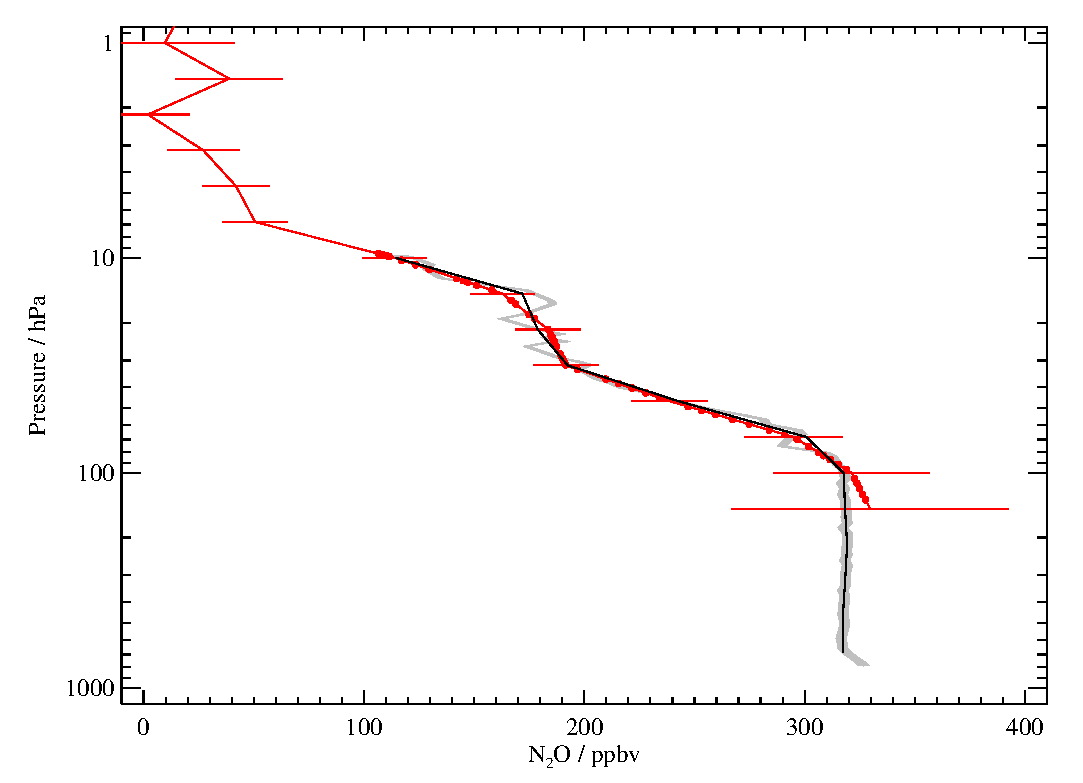
\includegraphics[width=\textwidth]{figures/basisexample}
  \caption{Comparisons of MLS (v1.5) N\cs2O observations with in-situ
    balloon data (courtesy of J.~Elkins).  The raw balloon data
    ($\b{z}_h$) are shown as the grey shaded region (shading indicates
    precision).  A coincident MLS profile ($\b{x}_l$) is shown in red with
    the red error bars indicating precision.  The red dots show the MLS
    data linearly interpolated to the balloon pressures using the $\b{H}$
    matrix (i.e., $\b{x}_h$ from equation~\ref{eqn:EtaForward}).  The
    black line shows the ``least squares'' interpolation of the balloon data
    onto the MLS grid using the $\b{W}$ matrix as described in the text
    (i.e., $\b{z}_l$ from equation~\ref{eqn:EtaBackward}).  The black line
    therefore represents the closest possible match at this resolution to
    the original grey line, and is the appropriate quantity to compare to
    the red MLS profile, and to be multiplied by the averaging kernels for
    formal comparison.}
  \label{fig:BasisExample}
\end{figure}

\section{A note on the HCl measurements in \thisv}

Starting in February~2006, the primary MLS band for measuring HCl (specifically the HCl\cp{35} isotopologue) (\texttt{R4:640.B13F:HCl} or ``band~13'') began to exhibit symptoms of aging and was deactivated to conserve life. This is likely to be due to a radiation susceptibility issue for a batch of transistors identified shortly before launch. Useful observations of HCl are still made with the adjacent band (\texttt{R4:640.B14F:O3} or ``band~14'') which, as can be seen from Figures~\ref{fig:UnfoldedSpectra} and~\ref{fig:FoldedSpectra} also observe the HCl\cp{35} line (and a smaller line for the HCl\cp{37} isotopologue); these retrievals produce the \thisv standard HCl product (as they did for earlier MLS data versions).

In order to avoid undesirable discontinuities in the \thisv HCl dataset, the band~13 radiances are not considered in the retrieval of the standard HCl product, even on days for which it was active. For days prior to the 16~February 2006 deactivation of band~13, and the few subsequent days when band~13 has been (or may be) reactivated, the \thisv algorithms also produce a second HCl product (in the \texttt{HCl-640-B13} swath in the \texttt{L2GP-DGG}) file which includes the band~13 radiances, giving a product with improved precision and resolution in the upper stratosphere and mesosphere. See Section~\ref{sec:StandardHCl} for more information.

As discussed in Section~\ref{sec:StandardHCl}, while the band~14 and band~13 data show very good agreement in the lower stratosphere, they disagree on the magnitude of the declining trend in upper stratospheric HCl (reflecting cuts in emissions of ozone depleting substances). At these high altitudes, the HCl line is significantly narrower than the single channel in band~14 in which it resides, whereas the band~13 channels (by design, as this band was targeted to HCl) resolve the line shape. Accordingly, the band~13 trend is judged to be the more accurate one.

\section{A note on \texorpdfstring{N\cs2O}{N2O} measurements in \thisv}

The originally preferred MLS band for measuring N\cs2O (band 12 in the 640\,GHz region, \texttt{N2O-640}) began to show signs of aging in June 2013 (although more slowly than the rapid decline observed in the HCl band~13 in 2006). Band~12 was subsequently turned off on August 6, 2013. For \thisv, as similarly for earlier versions, the band 3 (190\,GHz, \texttt{N2O-NitrousOxide}) retrievals are used as the standard product from launch, whereas the band 12 (640\,GHz, \texttt{N2O-640}) retrieval is now only available in the \texttt{N2O-640} swath in the \texttt{L2GP-DGG} file.

\section{A note on OH measurements in \thisv}
\label{sec:OHNote}

The MLS OH measurements derive from observations in the 2.5-THz region of the spectrum. The local oscillator signal driving the MLS 2.5-THz radiometers is provided by a methanol laser (pumped by a CO\cs2 laser). In December 2009, following more than five years of operation, this laser began to show signs of aging and was temporarily deactivated (prior to the 2004 Aura launch, the expected lifetime of this laser was only eighteen months).

Upper stratospheric and mesospheric OH is strongly affected by solar activity \citep{WangEtal:2013}, which was low during the solar 11-year minimum in 2009. In order to conserve the remaining lifetime of the THz instrument for valuable measurements when the Sun becomes more active, we suspended OH measurements from December 2009. The THz subsystem was reactivated for 30 day periods around August each year between 2011 and 2014, providing coverage of a full 11-year solar cycle. However, due to the aging of the instrument, OH data acquired in the 2014 period are significantly noisier than the previous years and have poor spatial coverage at mid-low latitudes. Any remaining life in the MLS THz subsystem is being conserved pending unusual solar activity.
